\chapter[Resultados Parciais]{Resultados Parciais}
\label{sec:resultados_parciais}

Com a conclusão da primeira etapa da pesquisa, algumas informações referentes a situação atual do projeto podem ser apresentadas. Com este objetivo, este capítulo se sub-divide nas seções de \textit{Revisão Sistemática}, \textit{Desenvolvimento prático} e \textit{Ações futuras}.

\section{Revisão Sistemática} % (fold)
\label{sec:revisão_sistemática}

	Com o objetivo de detalhar a revisão sistemática realizada durante esse trabalho de forma clara e objetiva, esta seção está divida nas seções de \ref{sub:planejamentoRevisao}, \ref{sub:conducaoRevisao} e \ref{sub:publicacaoRevisao}, seguindo o conceito apresentado por \cite{Kitchenham}, como mostra a figura \ref{img:processoGeralRevisao}.

	\begin{figure}[H]
			\centering
			\caption{Processo geral de revisão sistemática, segundo \cite{Kitchenham}}
			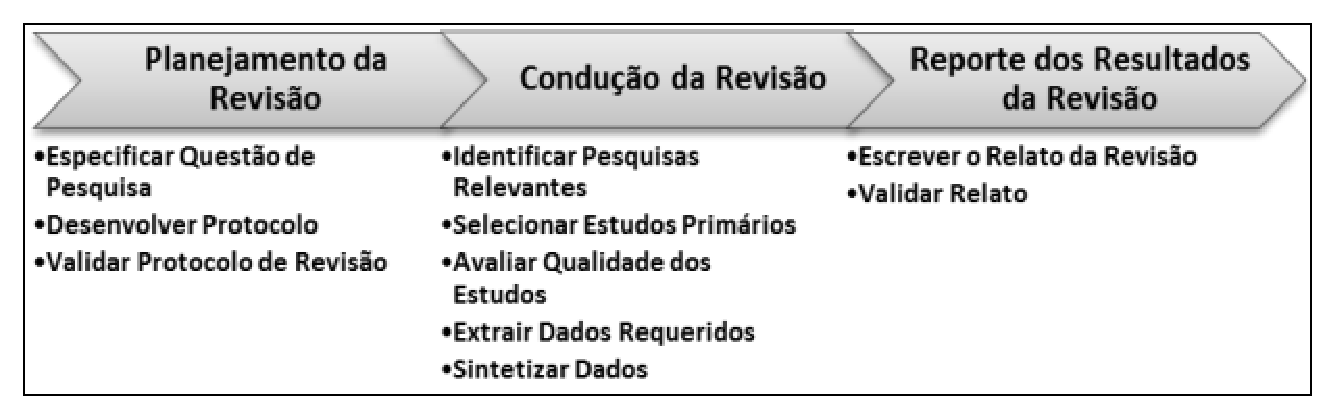
\includegraphics[scale=0.7]{figuras/processoGeralRevisao.eps}
			\label{img:processoGeralRevisao}
		\end{figure}

	\subsection{Planejamento da Revisão} % (fold)
	\label{sub:planejamentoRevisao}

		Esta revisão sistemática se deu entre os meses de março e junho de 2016, utilizando como fonte de busca as bases \textit{IEEE}, \textit{CAPES} e \textit{Springer}. A partir dos modelos de revisão sistemática apresentados por \cite{Kitchenham} e \cite{exemploRevisaoSistematica}, foi desenvolvido um protocolo de revisão, o qual possibilita, a outros pesquisadores, repetir a pesquisa.

		\subsubsection{Objetivos e questão de pesquisa}
		
		O objetivo inicial do trabalho é estudar a problemática da auto-localização na robótica, identificando diferentes soluções em diversos contextos. Afirmado isso, foi possível realizar uma pesquisa bibliográfica com o objetivo de identificar diferentes linhas de pesquisa nesta área. Após uma análise superficial de cada linha de pesquisa, foi selecionada a linha de pesquisa que adota, como solução para a auto-localização, a utilização da técnica de SLAM, o que pode ser considerado como o marco teórico do trabalho. 

		Com a identificação do marco teórico do trabalho, a definição do foco da pesquisa se torna uma tarefa menos árdua. Como o marco teórico deste trabalho se baseia nas linhas de pesquisa que buscam utilizar a técnica de SLAM para realizar navegação autônoma, esta revisão sistemática teve como objetivo identificar diferentes técnicas utilizadas atualmente para solucionar o problema de SLAM em diferentes contextos, desde contextos simplificados até contextos altamente complexos.

		A definição deste objetivo da revisão se dá pela necessidade de conhecimento amplo em relação a diferentes técnicas para solucionar o problema de SLAM. Como este trabalho buscará adaptar técnicas para um contexto simplificado, ou educacional, adicionou-se aos objetivos da revisão itens relacionados a robótica educacional e robôs simples.

		Segundo \cite{Kitchenham}, o primeiro passo para se realizar uma revisão sistemática é definir a sua questão de pesquisa. Desse modo, a partir da realização de uma pesquisa bibliográfica inicial, foram identificadas as seguintes questões de pesquisa: 

		\begin{itemize}
			\item \textbf{Q1}. \textit{Quais técnicas são mais utilizadas para solucionar o problema de SLAM?} e
			\item \textbf{Q2}. \textit{"Como tratar o problema de SLAM no contexto simplificado da robótica educacional?"}
		\end{itemize}

		Além das questões de pesquisa, de acordo com \cite{exemploRevisaoSistematica}, alguns outros itens devem ser detacados, como:

		\begin{itemize}
			\item \textbf{População}: comunidade acadêmica e de robótica.
			\item \textbf{Intervenção}: adaptação de técnicas para um contexto de robótica simplificado (educacional).
			\item \textbf{Controle}: utilização do \textit{Quasi-gold standard}.
			\item \textbf{Resultados}: obtenção de técnicas adaptáveis ao contexto simplificado.
			\item \textbf{Aplicação}: servir de base para a implementação da segunda etapa deste trabalho de conclusão de curso, onde técnicas serão adaptadas buscando solucionar, de maneira simplificada, o problema de SLAM.

		\end{itemize} 

		A partir da definição da questão de pesquisa e dos objetivos da revisão, buscou-se definir a estratégia de pesquisa, apresentada no tópico \ref{sub:estrategias_pesquisa}.

		\subsubsection{Estratégias de pesquisa}
		\label{sub:estrategias_pesquisa}

		A estratégia de pesquisa adotada para esta revisão segue recomendações de diversos autores, como \cite{Kitchenham} e \cite{systematicReviewEngSoft}, utilizando o conceito de \textit{quasi-gold standard}.

		Segundo \cite{quasi_goldES}, \textit{gold standard} representa o conjunto completo de estudos primários referentes a uma questão de pesquisa, com máxima precisão e sensitividade. Já o \textit{quasi-gold standard}, representa um subconjunto do \textit{gold standard}, o qual vai sendo evoluído ao longo dos ciclos de busca, com o objetivo de se aproximar do \textit{gold standard}. 

		É utilizado para definir os valores de precisão e sensitividade da busca, o que possibilita a avaliação da busca realizada, verificando a necessidade de refinamento da \textit{string}, por exemplo. \cite{quasi_goldES} define precisão e sensitividade da busca da seguinte forma:

		\begin{itemize}

			\item $precisão = \frac{ERO}{EO}$ e

			\item $sensitividade = \frac{ERO}{TER}$,
		\end{itemize}

		onde \textit{ERO} = número de estudos relevantes obtidos,
		
		\textit{EO} = número de estudos obtidos e

		\textit{TER} = número total de estudos relevantes.

		Esta definição possibilita a criação de critérios que avaliem a qualidade da busca, ou seja, da \textit{string} de busca utilizada. Porém, a seleção dos materiais deve seguir critérios relacionados a qualidade do material, os quais são divididos em \textit{critério de inclusão (CI)} e \textit{critério de exclusão (CE)}, como pode-se observar a seguir:

		\begin{itemize}
			\item CI 1 - Os artigos devem estar escritos em inglês ou português;
			\item CI 2 - Artigos referentes a auto-localização e mapeamento de ambientes simultâneos (SLAM);
			\item CI 3 - Artigos gratúitos e disponíveis na \textit{web} para \textit{download} ou leitura;
			\item CE 1 - Artigos que buscam solucionar o problema de auto-localização sem a utilização da técnica de SLAM;
			\item CE 2 - Artigos que tratem o tema de forma superficial. 
		\end{itemize}

		A partir da definição da questão de pesquisa e dos objetivos da revisão, assim como a definição dos critérios de inclusão e exclusão, foi possível desenvolver uma \textit{string} de busca inicial. O idioma escolhido para a \textit{string} de busca foi o inglês, devido a sua ampla utilização nas bases de conhecimento selecionadas. Buscou-se utilizar a mesma \textit{string} de busca em todas as bases de dados pesquisadas, exceto em alguns casos em que houve a necessidade da adaptação da \textit{string} de acordo com os padrões adotados pela base.


			Com o objetivo de identificar pesquisas relacionadas à auto-localização utilizando mapeamento de ambientes simultaneamente, a \textit{string} de busca definida foi: \textit{auto-localization AND environment mapping}. Na tabela \ref{tab:string_inicial} são apresentados os resultados obtidos a partir desta busca.

			\begin{table}[H]
			\centering
			\caption{Resultados obtidos com a \textit{string} inicial}
			\label{tab:string_inicial}
			\begin{tabular}{|c|c|c|}
			\hline
			\rowcolor[HTML]{C0C0C0} 
			\textbf{String}                                                                                    & \multicolumn{2}{c|}{\cellcolor[HTML]{C0C0C0}\textbf{IEEE, Springer e CAPES}}                                       \\ \hline
			                                                                                                   & \begin{tabular}[c]{@{}c@{}}Nº.\\ Artigos\end{tabular} & \begin{tabular}[c]{@{}c@{}}Nº.\\ Artigos\\ relevantes\end{tabular} \\ \hline
			\textit{\begin{tabular}[c]{@{}c@{}}Auto-localization \\ AND\\ environment \\ mapping\end{tabular}} & 29                                                    & 6                                                                 \\ \hline
			\end{tabular}
			\end{table}

		Esta primeira busca foi de extrema importância para se obter uma visão inicial da pesquisa, identificando novas palavras-chave e iniciando os ciclos de busca.


		% subsection subsection_name (end)

		\subsubsection{Procedimento de seleção}

			As buscas foram realizadas com a mesma \textit{string} de busca (na maioria dos casos, como já foi explicado anteriormente) nas três bases de conhecimento científico utilizadas. A cada busca realizada, os artigos foram registrados, para que, posteriormente, os mesmos pudessem ser submetidos à avaliação da qualidade e, se comprovada a relevância do mesmo, à extração de dados.

			A seleção dos artigos se deu a partir da leitura dos títulos, resumos e palavras-chave, classificando o artigo como relevante ou não, em um primeiro momento. Caso fosse confirmada a relevância do mesmo, o artigo passaria por uma avaliação mais profunda, a \textit{avaliação da qualidade}, como mostra o tópico \ref{sub:avaliacao_qualidade}.


		\subsubsection{Avaliação da Qualidade}
		\label{sub:avaliacao_qualidade}

			A avaliação da qualidade do artigo se deu a partir da análise do conteúdo do mesmo, focando principalmente na introdução, nos resultados e conclusões dos artigos. A avaliação positiva do artigo significa uma resposta positiva para as seguintes perguntas:

			\begin{enumerate}
				\item O estudo é interessante? (Em relação aos objetivos da pesquisa)
				\item As evidências apresentadas são válidas?
				\item As evidências apresentadas são importantes?
				\item As evidências apresentadas não contradizem nenhum autor selecionado como pilar da pesquisa?
			\end{enumerate}

			Com a confirmação da qualidade do material, o mesmo foi exposto à extração de dados, ou seja, a leitura completa e detalhada do artigo.

		\subsubsection{Extração de dados}

			Com o objetivo de organizar os dados obtidos, facilitando o manuseio das informações, os dados extraídos de cada artigo foram registrados a partir da utilização do padrão apresentado no exemplo da tabela \ref{tab:padrao_dados_extraidos}, além do detalhamento mais aprofundado do material a partir da criação de um resumo informal do artigo.

			\begin{table}[H]
				\centering
				\caption{Exemplo de registro de material}
				\label{tab:padrao_dados_extraidos}
				\begin{tabular}{|c|c|c|c|l|}
					\hline
					\rowcolor[HTML]{C0C0C0} 
					\textbf{Título}                                                                                                                                    & \textbf{Autor(es)}                                                                                    & \textbf{\begin{tabular}[c]{@{}c@{}}Data de\\ publicação\end{tabular}} & \textbf{\begin{tabular}[c]{@{}c@{}}Fonte da\\ publicação\end{tabular}} & \multicolumn{1}{c|}{\cellcolor[HTML]{C0C0C0}\textbf{\begin{tabular}[c]{@{}c@{}}Listagem das\\ informações\\ importantes\end{tabular}}} \\ \hline
					\textit{\begin{tabular}[c]{@{}c@{}}Integration of Vision\\ based SLAM and \\ Nonlinear Filter for\\ Simple Mobile Robot\\ Navigation\end{tabular}} & \begin{tabular}[c]{@{}c@{}}Dae Hee Won,\\ Young Jae Lee,\\ Sangkyung Sung,\\ Taesam Kang\end{tabular} & 2008                                                                  & IEEE                                                                   & \begin{tabular}[c]{@{}l@{}}-Utilização de\\ sensor de visão\\ e encoders.\\ -Filtro de \\ partículas\end{tabular}                      \\ \hline
				\end{tabular}
			\end{table}

		
	% subsection planejamento_da_revisão (end)

	\subsection{Condução da Revisão} % (fold)
	\label{sub:conducaoRevisao}
		
		Durante a condução da revisão, a busca efetiva dos materiais é realizada, os ciclos de busca são documentados e a \textit{string} de busca é refinada, como afirma \cite{estudoPrimarioSecundario}.

		Esta pesquisa foi realizada entre os meses de março e junho de 2016. A \textit{string} de busca apresentada no tópico \ref{sub:estrategias_pesquisa} resultou em uma visão considerada fraca, pelo pesquisador e seus orientadores, sobre a auto-localização e o mapeamento de ambientes, peças chave da técnica de SLAM. Além disso, essa busca possibilitou a criação do \textit{quasi-gold standard} inicial, com apenas um artigo: \textit{Auto-localização e construção de de mapas de ambiente para robôs móveis baseados em visão omnidirecional estéreo} \cite{localizacaoEMapeamentoPaulo}. 

		Desse modo, foi necessária a realização de uma pesquisa manual para obter maior conhecimento sobre o tema e as palavras-chave a serem usadas para garantir maior qualidade dos resultados obtidos. Com a realização desta pesquisa, os seguintes artigos foram adicionados ao \textit{quasi-gold standard}:

		\begin{itemize}
			\item \textit{The Cleaning Robot Project: Aplicação do Filtro de Kalman na Auto-Localização de um Sistema Robótico Autônomo} \cite{theCleaningProject},
			\item \textit{Integration of Vision based SLAM and Nonlinear Filter for Simple Mobile Robot Navigation} \cite{integrationVisionSLAMnonlinear} e
			\item \textit{A Solution to the Simultaneous Localization and Map Building (SLAM) Problem} \cite{slamProblem}.
		\end{itemize}

		A partir da análise destes artigos inciais, foi possível identificar diversas palavras-chave que levavam à pesquisa desejada, possibilitando refinamento da \textit{string} de busca. Adicionando à mesma novos termos, como \textit{"SLAM problem"} e \textit{"simultaneous"}, evoluindo a \textit{string} e obtendo o seguinte resultado: \textit{"simultaneous AND auto-localization AND environment mapping AND SLAM problem"}.
		
		O ciclo de busca utilizando esta \textit{string} gerou poucos resultados, selecionando apenas um para análise: \textit{Improved global localization of an indoor mobile robot via fuzzy extended information filtering} \cite{ROB:1764504}. Com o objetivo ampliar abrangência da busca, optou-se por modificar a palavra-chave \textit{auto-localization} por apenas \textit{localization}, obtendo a seguinte \textit{string} de busca: \textit{"simultaneous AND localization AND environment mapping AND SLAM problem"}.

		Com a realização deste novo ciclo de busca, diversos artigos relevantes foram identificados e adicionados ao \textit{quasi-gold standard}. Os artigos presentes no \textit{quasi-gold} corrente foram encontrados com esta nova busca, evidenciando uma certa qualidade da \textit{string} de busca. Os artigos adicionados ao \textit{quasi-gold standard} durante este ciclo são:

		\begin{itemize}
			\item \textit{A Simultaneous Localization and Mapping Algorithm in Complex Environments: SLASEM} \cite{slasem},
			\item \textit{A Neuro-Fuzzy Assisted Extended Kalman Filter-Based Approach for Simultaneous Localization  and  Mapping (SLAM) Problems} \cite{neurofuzzi},
			\item \textit{Map Management for Efficient Simultaneous Localization and Mapping (SLAM)} \cite{mapManagement} e
			\item \textit{Simultaneous Localization and Map Building by Integrating a Cache of Features} \cite{integratingCacheFeat}.
		\end{itemize}

		Com o intúito de especificar mais a busca, foi adicionada, devido a uma dica do orientador prof. Dr. Maurício Serrano, a palavra-chave \textit{"simple robots"} à \textit{string} de busca, chegando a seguinte \textit{string}: \textit{"simultaneous AND localization AND environment mapping AND SLAM problem OR ("simple mobile robots" AND slam)"}.

		Com esta mudança, obteve-se uma outra visão desta pesquisa como um todo, foram identificadas diversas pesquisas que buscam solucionar problemas de locomoção, como o problema de SLAM, em contextos limitados, da mesma forma que objetivo geral deste trabalho. Dessa forma, foram adicionados ao \textit{quasi-gold standard}, os seguintes artigos:

		\begin{itemize}
			\item \textit{BatSLAM: Simultaneous Localization and Mapping Using Biomimetic Sonar} \cite{batslam},
			\item \textit{Neural Network-Based Multiple Robot Simultaneous Localization and Mapping} \cite{neuralNetwork} e
			\item \textit{Visual simultaneous localization and mapping: a survey} \cite{surveyLocalization}.
		\end{itemize}

		Como é possível observar, os artigos selecionados para adição no \textit{quasi-gold standard} não envolviam temas referentes a robôs simples, apesar da afirmação de que esta mudança havia modificado a visão da pesquisa. Artigos referentes a este tema não foram adicionados ao \textit{quasi-gold standard} devido ao fato dos mesmos serem \textit{barrados} pelo critério de exclusão \textit{"CE 2 - Artigos que tratem o tema de forma superficial"}. 

		Em contrapartida, este ciclo possibilitou o conhecimento de novos termos, viabilizando um refinamento eficiente para o próximo ciclo de busca.

		No próximo ciclo de busca, foram adicionadas palavras-chave referentes a robótica educacional e estratégias de resolução do problema de SLAM, como mostra a \textit{string}: \textit{"(Simple mobile robot? AND (SLAM OR auto-localization)) AND (map* OR education* robot*) AND strateg*"}. Além de adicionar estes novos termos, utilizou-se de técnicas disponíveis nas bases, como a utilização de \textit{'?'}, que representa qualquer caractere, e \textit{*}, que significa que quaisquer caracteres precedidos dos caracteres anteriores ao \textit{*} serão considerados.

		Para realização desta busca, foi necessária a adaptação da \textit{string} de busca durante a pesquisa na base de dados \textit{Springer}, devido a diferenças nos padrões de definição da \textit{string}. Para esta adaptação, novas palavras-chave precisaram ser selecionadas, as quais foram obtidas a partir dos resultados advindos das outras bases, com a mesma \textit{string}.

		A \textit{string} adaptada para a base \textit{Springer} foi: \textit{"(Simple AND mobile AND robot AND SLAM AND localization AND mapping) AND (educational AND navigation AND simultaneous) AND strategies"}.

		Ao realizar esta busca, foi observado que os resultados atendiam, em sua maioria, ao desejado pela pesquisa, muitos artigos foram selecionados para análise e avaliação e alguns foram adicionados ao \textit{quasi-gold standard}, como:

			\begin{itemize}
				\item \textit{Incremental SLAM with Backtracking Data Association for Mobile Robots} \cite{incrementalSLAM},
				\item \textit{Mapping and Pursuit-Evasion Strategies For a Simple Wall-Following Robot} \cite{wall_following} e
				\item \textit{A Simple and Parallel Algorithm for Real-Time Robot Localization by Fusing Monocular Vision and Odometry/AHRS Sensors} \cite{fusingSensorsParallel}.
			\end{itemize}

		Com a realização desta busca, foram obtidos 27 artigos, restando apenas 20 após a avaliação da relevância dos mesmos para a pesquisa. Desde o primeiro ciclo de busca, diversos artigos foram considerados relavantes para a pesquisa, chegando a um número de 42 (quarenta e dois) artigos relevantes.
		
		Ou seja, aplicando os conceitos de \textit{precisão} e \textit{sensitividade}, temos que:

		\begin{itemize}
			\item $sensitividade = \frac{20}{42}$ e
			\item $precisao = \frac{20}{27}$
		\end{itemize}

		Desse modo, foi obtida uma \textit{sensitividade} de 47\% e uma precisão de 74\%, dando fim aos ciclos de busca com 42 artigos selecionados e analisados. A tabela \ref{tab:string_final} apresenta, de maneira resumida, a evolução da \textit{string} de busca, comparando a \textit{string} inicial com a \textit{string} final da pesquisa.

\begin{table}[H]
\centering
\caption{Comparação das \textit{strings} inicial e final}
\label{tab:string_final}
\begin{tabular}{|c|c|c|c|c|}
\hline
\multirow{2}{*}{\textbf{String}} & \multirow{2}{*}{\textbf{\begin{tabular}[c]{@{}c@{}}Fonte de \\ busca\end{tabular}}} & \multicolumn{2}{c|}{\textbf{Resultados}} & \multirow{2}{*}{\textbf{Observações}}                                                                                                                                                        \\ \cline{3-4}
                                 &                                                                                     & \textbf{Total}   & \textbf{Relevantes}   &                                                                                                                                                                                              \\ \hline
\multirow{3}{*}{Inicial}         & \textit{IEEEXplore}                                                                 & 2                & 1                     & \multirow{3}{*}{\begin{tabular}[c]{@{}c@{}}String construída sem o conhecimento\\ necessário para utilização das palavras-\\ chave que representam a pesquisa.\end{tabular}}                 \\ \cline{2-4}
                                 & \textit{Springer}                                                                   & 19               & 2                     &                                                                                                                                                                                              \\ \cline{2-4}
                                 & \textit{CAPES}                                                                      & 8                & 3                     &                                                                                                                                                                                              \\ \hline
\multirow{3}{*}{Refinada}        & \textit{IEEEXplore}                                                                 & 17               & 13                    & \multirow{3}{*}{\begin{tabular}[c]{@{}c@{}}String refinada, ao longo de diversos ciclos de \\ busca, adicionando novas palavras-chave e\\ obtendo resultados mais específicos.\end{tabular}} \\ \cline{2-4}
                                 & \textit{Springer}                                                                   & 6                & 3                     &                                                                                                                                                                                              \\ \cline{2-4}
                                 & \textit{CAPES}                                                                      & 4                & 4                     &                                                                                                                                                                                              \\ \hline
\end{tabular}
\end{table}

Durante a realização de cada ciclo, os artigos foram analisados, avaliados e seus dados foram extraídos como fonte de estudo para a realização deste trabalho de conclusão de curso. Na seção \ref{sub:publicacaoRevisao} serão apresentados os resultados de maneira organizada e simplificada.

		% subsection condução_da_revisão (end)

	\subsection{Publicação dos Resultados} % (fold)
	\label{sub:publicacaoRevisao}
		
		A primeira etapa deste trabalho de conclusão de curso pode ser vista como o resultado geral desta revisão sistemática, onde conceitos, termos, abordagens e qualquer informação utilizada no trabalho é fruto, seja direta ou indiretamente, desta revisão sistemática.

		Com o objetivo de documentar os resultados diretos desta revisão sistemática, estes foram registrados como as técnicas utilizadas atualmente para solucionar o problema de SLAM em diferentes contextos. 

		Com a realização desta revisão, foi possível identificar \textit{áreas} mutáveis nas diferentes soluções do problema de SLAM. As áreas identificadas são \textit{"arquitetura da solução"} \ref{sub:arquitetura_solucao}, \textit{"técnica probabilística utilizada"} \ref{sub:prob_usada} e \textit{"informações disponíveis"} \ref{sub:infos_disponiveis}. Em cada solução, os autores buscaram se adequar ao contexto trabalhado, seja a partir da disponibilidade de sensores específicos ou da capacidade computacional disponível.

		Como uma forma de organizar os resultados obtidos, os mesmos serão sub-divididos nas áreas citadas acima, apresentando conceitos, vantagens e desvantagens da utilização de cada técnica.

		\subsubsection{Arquitetura da solução}
		\label{sub:arquitetura_solucao}

			A arquitetura da solução, na grande maioria dos estudos, foi definida a partir do requisito computacional. Ou seja, a limitação computacional presente nos robôs simples levou os autores a buscarem arquiteturas que contornassem esse problema, como mostra \cite{redeComunicacaoIndustria}. Entre as diversas arquiteturas, as mais comumente utilizadas são as que buscam processar as informações em um computador, utilizando o robô apenas para obtenção das informações, como ilustra a figura \ref{img:arquitetura_mais_utilizada}.

			\begin{figure}[H]
				\centering
				\caption{Arquitetura de comunicação}
				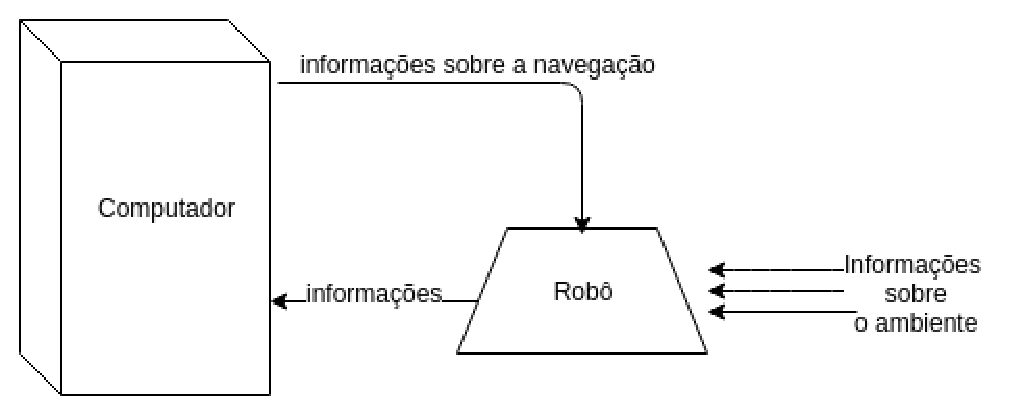
\includegraphics[scale=0.9]{figuras/arquitetura_mais_utilizada.eps}
				\label{img:arquitetura_mais_utilizada}
			\end{figure}

			De acordo com a figura \ref{img:arquitetura_mais_utilizada}, o robô será responsável apenas por obter informações do ambiente, ou seja, recuperar os dados obtidos a partir dos sensores disponíveis. O computador, em posse das informações sobre o ambiente, ou seja, os pontos de referência, a quantidade de rotações em cada roda, a distância e cores de objetos, por exemplo, será responsável por processar toda a informação, construindo um mapa lógico para possibilitar a localização do robô em relação ao ambiente, como apresenta \cite{redeComunicacaoIndustria}.

			Geralmente, são utilizados dois mapas simultâneos, um presente no robô (local) e outro, mais completo, presente no computador (remoto). O mapa local é, basicamente, um vetor de pontos \textit{'p'} em relação a um tempo \textit{'t'}, como explica \cite{circumventingAssociationSLAM}. O computador utiliza este mapa local, que é disponibilizado pelo robô, para completar, corrigir e atualizar o mapa remoto, mesclando informações e utilizando, geralmente, filtros probabilísticos para maximizar sua precisão \cite{localizacaoEMapeamentoPaulo}.

			As decisões referentes à navegação são geradas a partir da análise do mapa remoto, já que o mapa local é incompleto e inconsistente, como afirma \cite{redeComunicacaoIndustria}. A utilização desta arquitetura de mapeamento remoto e local torna prática a realização de navegações com múltiplos robôs, como apresenta, \cite{redeComunicacaoIndustria}, em seu trabalho sobre rede de comunicação sem fio para navegação de múltiplos robôs. 

			Seguindo esta arquitetura, \cite{neuralNetwork} e \cite{multiRobots} também desenvolveram sistemas de resolução do problema de SLAM com a utilização de múltiplos robôs, mostrando a viabilidade da sua utilização. Neste tipo de trabalho, os robôs colaboram entre si, pois, como a informação obtida é centralizada em um computador único, as decisões referentes à navegação de um determinado robô são resultados do processamento das informações obtidas por todos os robôs, maximizando a vizão global de cada robô \cite{redeComunicacaoIndustria}.

			De qualquer forma, independente da arquitetura da solução utilizada, os erros advindos dos sensores sempre serão um problema sério a ser resolvido \cite{circumventingAssociationSLAM}. Com o objetivo de solucionar este problema, a comunidade de robótica se vê presa à utilização de estruturas matemáticas probabilísticas, como afirma \cite{circumventingAssociationSLAM}. As seções \ref{sub:kalman}, \ref{sub:filtro_de_partículas} e \ref{sub:prob_usada} apresentam as estruturas probabilísticas mais utilizadas atualmente, assim como suas vantagens e desvantagens.

		\subsubsection{Técnica probabilistica utilizada}
		\label{sub:prob_usada}

			

			Qualquer técnica que busque solucionar o problema de SLAM precisa, assim como praticamente toda a robótica, de filtros probabilísticos para minimizar o erro das informações obtidas pelos sensores. Entre estes filtros, estão o filtro de Kalman, apresentado na seção \ref{sub:kalman}, e o filtro de partículas, apresentado na seção \ref{sub:filtro_de_partículas}. 

		\subsubsection{Informações disponíveis}
		\label{sub:infos_disponiveis}

			Na robótica móvel, existem diversas maneiras de se obter informações sobre o ambiente, a partir da utilização de sensores específicos para informações específicas. Entre os sensores mais utilizados, se encontram os \textit{sonares, sensores de infra-vermelho, câmeras de vídeo, sensores de distância, sensores RGB e sensores odométricos}. A partir do ambiente em que se deseja navegar, faz-se necessária a seleção dos sensores adequados para o contexto.

			Porém, como foi explicado no tópico \ref{sub:prob_usada}, os sensores possuem margens de erro que muitas vezes podem prejudicar a navegação. Em busca de tentar solucionar este problema, além da utilização de filtros probabilísticos, diversos autores utilizaram múltiplos sensores, integrando as informações dos mesmos para que cada sensor colaborasse na calibração do outro sensor. 
	% subsection publicação_dos_resultados (end)

% section revisão_sistemática (end)

\section{Desenvolvimento prático} % (fold)
\label{sec:desenvolvimento_prático}

	Apresentar detalhes sobre a utilização de ferramentas, conhecimentos obtidos com a prova de conceito, problemas encontrados, soluções e etc.
% section desenvolvimento_prático (end)

\section{Ações futuras} % (fold)
\label{sec:acoes_futuras}

	Durante a segunda etapa do trabalho, pretende-se evoluir a prova de conceito apresentada durante esta primeira etapa, buscando solucionar, de maneira simplificada, o problema de SLAM. A partir dos ciclos de desenvolvimento, serão realizadas análises referentes às peculiaridades encontradas ao implementar uma técnica de auto-localização em robôs simples, assim como o impácto desta implementação em um contexto educacional.

% section section_name (end)